% This template was initially provided by Dulip Withanage.
% Modifications for the database systems research group
% were made by Conny Junghans,  Jannik Strtgen and Michael Gertz

\documentclass[
     12pt,         % font size
     a4paper,      % paper format
     BCOR=10mm,version=first,     % binding correction
     DIV=14,version=first,        % stripe size for margin calculation
%     liststotoc,   % table listing in toc
%     bibtotoc,     % bibliography in toc
%     idxtotoc,     % index in toc
%     parskip       % paragraph skip instad of paragraph indent
     ]{scrreprt}

%%%%%%%%%%%%%%%%%%%%%%%%%%%%%%%%%%%%%%%%%%%%%%%%%%%%%%%%%%%%

% PACKAGES:

% Use German :
\usepackage[english]{babel}
% Input and font encoding
\usepackage[utf8]{inputenc}
\usepackage[T1]{fontenc}
% Index-generation
\usepackage{makeidx}
% Einbinden von URLs:
\usepackage{url}
% Special \LaTex symbols (e.g. \BibTeX):
%\usepackage{doc}
% Include Graphic-files:
\usepackage{graphicx}
% Include doc++ generated tex-files:
%\usepackage{docxx}
% Include PDF links
%\usepackage[pdftex, bookmarks=true]{hyperref}
\usepackage{csquotes}

% Fuer anderthalbzeiligen Textsatz
\usepackage{setspace}

% hyperrefs in the documents
\usepackage[bookmarks=true,colorlinks,pdfpagelabels,pdfstartview = FitH,bookmarksopen = true,bookmarksnumbered = true,linkcolor = black,plainpages = false,hypertexnames = false,citecolor = black,urlcolor=black]{hyperref} 
%\usepackage{hyperref}


%%%%%%%%%%%%%%%%%%%%%%%%%%%%%%%%%%%%%%%%%%%%%%%%%%%%%%%%%%%%

% OTHER SETTINGS:

% Pagestyle:
\pagestyle{headings}

% Choose language
\newcommand{\setlang}[1]{\selectlanguage{#1}\nonfrenchspacing}

\usepackage{biblatex}
\addbibresource{references.bib}

\begin{document}

% TITLE:
\pagenumbering{roman}
\begin{titlepage}
     \vspace*{1cm}
     \begin{center}
          \vspace*{3cm}
          \textbf
          {
               \Large University of Heidelberg\\
               \smallskip
               \Large Institute for Computer Science\\
               \smallskip
               \Large Working group database systems\\
               \smallskip
          }

          \vspace{3cm}

          \textbf{\large Bachelor thesis}

          \vspace{0.5\baselineskip}
          {
               \huge
               \textbf{Integrating Identity Management Providers based on Online Zugangs Gesetz}
          }

     \end{center}

     \vfill
     {
          \large
          \begin{tabular}[l]{ll}
               Name:                 & Jonas Gann              \\
               Matriculation number: & 3367576                 \\
               Supervisor:           & Prof. Dr. Michael Gertz \\
               Date of submission:   & \today
          \end{tabular}
     }

\end{titlepage}

\onehalfspacing

\thispagestyle{empty}

\vspace*{100pt}
\noindent
I assure that I have written this bachelor thesis on my own and only used the specified sources and resources and that I followed the principles and recommendations "Responsibility in Science" of the University of Heidelberg.

\vspace*{50pt}
\noindent

\underline{\phantom{mmmmmmmmmmmmmmmmmmmm}}

\medskip
\noindent
Date of Submission: \today
\newpage

\chapter*{Zusammenfassung}

\newpage

\chapter*{Abstract}

\newpage

\tableofcontents
\cleardoublepage
\pagenumbering{arabic}

\chapter{Context}
Since invention of the World Wide Web, the number of its users increased rapidly. Today, more than 90 percent of the German population use the internet \cite{Onlinestudie}. Enterprises and organizations, recognised this potential to provide their services to a large number of people as Service Providers (SP). A frequently used method of SPs is "online self-service" (OSS). Specialized software tools enable customers to use services through the internet without direct human interaction.

Many tools require identification of a user in case interactions or initiated business processes have to be associated with him. A system for management of identities of users therefore is part of numerous system architectures. Service Providers usually enable users to manage their partial identities using online self-service through so called User Profiles. Today, customers of SPs are associated with multiple partial identities and user profiles - one for each SP

The result is variety of problems in management of digital identities \cite{IdentityCrisis}. Here are some examples:
\begin{itemize}
    \item Multiple SPs collect, use and share parts of identities which leads to distributed and fragmented identities.
    \item As a result of the distributed identities, risk of data breaches increases.
    \item Managing multiple use profiles is very inconvenient for users.
    \item It is often unclear who stores which data and for what purpose.
    \item SPs have an incentive to collect and share more user data than they need.
\end{itemize}

An improved model for identity management is necessary. In recent years, multiple new models have been invented. One model called Social Login became popular. It enables customers to create User Profiles for SPs through existing User Profile of Social Networks like Facebook. This improves identity management by enabling SPs to rely on the external profile for unique identification, authorisation and personal attributes. Users can therefore manage identity related information through their Social Profile which is accessed by the SP.

This approach, however, still leaves the requirement of User Profiles for each SP because, depending on the provided service, additional attributes which are not part of the Social Profile, have to be manageable by the user. SPs also might require additional online self-service tools the social network does not provide.

The solution to this problem is an Identity Management Provider (IMP) which manages the whole online identity of a person and can replace the individual partial identities and User Profiles. The system itself is provided and hosted by a SP for consumption by other SPs. To replace existing User Profiles, the IMP can not only rely on systems for registration, authentication, authorisation and provisioning. Additional requirements of SPs like communication, data wallet and management of additional attributes have to be satisfied.

In order for an SP to use identities and services of an IMP, an integration into the system architecture of the SP has to take place. Due to the complex nature of system architectures and identity management, this is a difficult task.

A currently relevant example for usage of online self-service with particular interesting requirements for identities is the German "Online Access Law" (Online Zugangs Gesetz: OZG). It requires all administrative services of the German federal republic, each member state and commune to be digitally available through interoperable user profiles. The current plan is to make the profiles only available for usage in context of the OZG. From a user perspective, this would be yet another partial identity and user profile to manage.

\chapter{Objective}
Based on the prominent example of the OZG, the bachelor thesis will construct a message based integration architecture which enables system architectures of service providers with existing user profiles to make their services usable with an Identity Management Provider. In order to make the integration architecture suitable to real life requirements, the OZG is selected as an example due to its current relevance and high requirements regarding identity management. The integration architecture is however not only applicable in cases relevant for OZG but also for other Service Providers with similar requirements. As requirements of SPs are not guaranteed to be similar to those of the OZG, the integration architecture is built to be expendable.

The \textbf{integration architecture} for the OZG enables \textbf{IMP functionalities} to be usable for selected \textbf{OZG scenarios} by integrating a \textbf{connector} in the \textbf{system architecture} of a member state.

\begin{itemize}
    \item OZG scenarios are based on documented digitalization efforts of administrative services in the context of the OZG and are for example the application for an administrative service or the communication with a governmental institution.
    \item The system architecture is based on documentation about architecture plans of member states.
    \item The functionalities of the IMP are based on a requirements analysis of OZG scenarios and additional research.
    \item The connector is defined based on functionalities the integration architecture requires from the IMP.
    \item The integration architecture is the main scientific contribution of this bachelor thesis. It is based on messaging patterns in order to utilize a combination of established and tested messaging solutions. In order to save investments it also reuses as many system components as possible and modifies as few system components as necessary.
\end{itemize}

The integration architecture ...

\chapter{Structure of Work}
The "Fundamentals" chapter explains terminology and basic concepts.

In the following chapter called "Identity Management System" the thesis analyzes requirements for identity management through the perspective of the user and through the perspective of service providers for the OZG. It is presented, how an identity management provider could solve current identity management problems and which challenges for an integration exist.

The chapter "Integration Proposal" first documents a possible IMP system and connector, based on the requirement analysis of the previous chapter. It then presents the integration architecture with iteratively increasing requirements through textual description, multiple flow diagrams and messaging architectures.

A "Solution Evaluation" analyzes benefits and problems of the proposed solution.

The "Outlook" will conclude the thesis by presenting possibilities for advanced integration architectures.

\chapter{Fundamentals}

\section{Terminology}

\paragraph{Service Provider}
Service providers (SP) are entities like enterprises or organisations which make services accessible over the internet.

\paragraph{Online Self-Service}
Online self-service (OSS) describes a method used by Service Providers to make their services available to the user. The method is characterized by being available over the internet, requiring no direct human interaction but instead enabling the user to access services in a self-reliant way. The user is usually supported by a variety of software solutions.

\paragraph{Self-Service Tools}
Self-service tools are software solutions for customers to enable a online self-service experience. Depending on the use case, the tools can be transactional or informing. Informing tools help users to retrieve relevant information, often replacing human customer support. Transactional tools help users to interact with services in a persistent way to for example save personal data or trigger business processes.

Information tools can be for example so called "WiKi" pages or search fields which assist the user in his process of finding information. Transactional tools can be for example online forms which assist the user in his process of triggering an order placement business process.

In contrast to information tools, transactional tools often require identification of users in order to associate them with changes they made to the system: If a user triggers the business process of ordering a product, the SP requires identification of the user.

\paragraph{Digital Identity}
The digital identity, for simplicity called identity in the thesis, is the sum of all digital personal information. Each piece of personal information is an attribute. Attributes can be identifiers which are able uniquely identify an entity. It is also possible to use an aggregation of attributes as identifier.

Identifiers which are commonly used by SPs are the phone number and E-Mail address. Attributes are for example nicknames, hobbies, interests or education. The full name of a person is often not sufficient unique identification, the aggregation of name, age and home address can therefore be used as identifier.

\paragraph{Partial Digital Identity}
A partial digital identity is a subset of an identity. Partial identities are commonly used by SPs to manage identity information which is relevant for them. 

\paragraph{Identity Management}
Identity management is the creation, utilization / reading , updating and deletion of identities or partial identities. The possible utilization of identities depends on the system for management of identities. It could be for example authorization for a service or communication through an inbox.

\paragraph{Identity Management System}
Identity management systems are solutions which enable SPs and customers to manage identities or partial identities.
They usually provide the following functionalities an properties:
\begin{itemize}
    \item 
\end{itemize}

\paragraph{User Profile}
User profiles are one method for identity management. They are characterized by each SP providing a separate identity management system which often consist of an identity provider (IdP) for storing identities, a customer relation management system (CRM) for accessing identities internally and a website with online self-service tools for providing access to customers.

\section{Identity Management Provisioning (IMP)}
Identity management provisioning (IMP) is a method for identity management which is characterized by an identity management provider hosting an identity management system for "non-partial" identities. The identity management system provides one-stop online self-service for users and manages the storage of identities. SPs are provided access to the identities of the identity management system.

The following are functionalities of an IMP system in addition to those of conventional identity management systems:

\paragraph{Attribute Management}
It is common for identity management systems to enable users to manage a predetermined set of attributes. IMP systems however do not just manage partial identities and therefore enable users to manage any possible attribute of their identity. Users therefore can add, remove and modify any attribute.

As often, attributes of a digital identity are defined by service providers, they are also able to create new attributes or delete and modify existing ones, if approved by the user. 

\paragraph{Online Self-Service}
Many attributes, especially those created by SPs, do not make sense to the user without context and my be heavily dependant on systems of a SP. Therefore, the IMP provides solutions for online self-service which supports the management of attributes.

\paragraph{Integration}
Service providers which use IMP systems as solution for identity management require access to its services and have to make their existing systems work with them. The IMP solution therefore provides interfaces which enable the SP to access services. As it is in the best interest of the IMP solution to integrate SPs, advanced integration methods reducing the integration effort for SPs can be provided. 

\section{Online Access Law (OZG)}
In 2017 the German government passed the law for improvement of online access to administrative services (Online Zugangs Gesetz: OZG) which requires federal republic and member states to execute the following regulations until 2022 \cite{BMI:OZG_Wortlaut}:
\begin{enumerate}
    \item \textbf{Digital availability of administrative services} \\
    An administrative service is the electronic processing of administrative procedures which are available from outside the governmental institution.  As it is not clear which administrative services exactly are meant by the definition of the OZG, the BMI created a catalogue \cite{BMI:Verwaltungsleistungen}. The OZG requires these services to be digitally available. As a guideline to what is considered sufficient availability, the BMI defined a maturity model \cite{BMI:Digitale_Services}.
    \item \textbf{Digital access to administrative services through administration portals of a portal network} \\
    Federal republic, each member state and each commune must provide an administration portal. Portals of communes must be linked to the portal of the corresponding member state. Portals of federal republic and member states must be connected through a portal network. \cite{BMI:Portalverbund} Each portal must provide a "seek and find" feature, which enables users to find all administrative services provided by any administration portal \cite{Cotar:Drucksache_19/19089}. 
    \item \textbf{Interoperable user profiles for accessing administrative services} \\
    Federal republic and member states must provide user profiles which can be used to identify the corresponding person while requesting access to administrative services, to save personal information according to the once-only principle, to receive and send messages via a digital mailbox and to pay for services \cite{Cotar:Drucksache_19/19089}. The user profiles must be interoperable for every administration portal of the portal network.
\end{enumerate}

Execution of the OZG can be separated into two projects:

\paragraph{Digitalization}
Digitalization of administrative services focuses on accessibility towards users but not modernization of its internal execution by administrative institutions. The goal of digitalization in this case is, to make administrative services available towards a user in a digitized way:

A digitized administrative service can be accessed by a user through a website. The website is hosted either by the federal republic or a member state and is called "Administration Portal". Access is usually provided through an application form. The administrative service can be managed through a user profile which is provided by the federal republic or the member state. Management of an administrative service usually includes starting the service by sending in a form, communicating with responsible institutions through the inbox of the profile and receiving a result. The user profile can also enable users to upload documents to a data wallet and to save personal information for automatically filling in forms.

Digitalization of an administrative service is the modification of the underlying processes to incorporate the usage of the described features of the user profile and administration portal. In total, the BMI lists 575 relevant services, some of them provided by the federal republic, some by the member states and yet other by the communes \cite{BMI:Onlinezugangsgesetz}.

\paragraph{Networking}
The networking focuses on connecting governmental systems to make all digitized administrative services available for every user. This includes most importantly the connection of administration portals to a portal network through an online gateway and the interoperability of user profiles.

In order to save investments a method called "one for all" is used when hosting administrative services. One member state or the federal republic provide access to a service on their administration portal and distribute the requests to the responsible institutions "under the hood". As administration portals are connected through an "online gateway", each portal contains a search feature, which enables users to find all administrative services through any portal. Interoperable user profiles enable usage of each profile for management of administrative services on all portals.

\subsection{Administrative Service}
Unemployment benefit (Arbeitslosengeld II: AGII) is selected as an example for a digitized administrative service, because it has a high priority according to the "OZG-Informationsplattform" and is well documented.

The AGII is accessible through the "one for all" method through the administration portal of the federal republic. The digitalization of the service was done by the member state Nordrhein-Westfalen. The purpose of this service is to enable application for unemployment benefit and the result is an approval or denial by the responsible institution of the commune. The digitized process of this service enhances it to be manageable on an administration portal trough a user profile in the following way:

In order to access the service, a user must authenticate for an existing user profile or create one.

\subsection{System Architecture}
This subsection describes the system architecture of a member state relevant for the execution of the OZG.

\subsubsection{System Components}
The system architecture consists of the following system components where each component is responsible for processing a certain group of tasks:

\paragraph{User Profile}
Each member state provides its own user profile which manages the identity of a user. It enables him to create, delete and login to a profile, authenticate for administration services, communicate with institutions through an inbox and manage personal information and documents in a data wallet.

\paragraph{Administration Portal}
The administration portal provides the user with a web-interface he can use to access his user profile and search for available administration services.

\paragraph{Application Platform}
The application platform gives access to administration services by providing the user with a website he can use to fill in application forms and sent them to the responsible institutions. It is possible to prefill the form with personal data stored inside the user profile.

\paragraph{Institution}
Institutions are the entities distributed all over the member state which eventually process the incoming applications and provide the users with solutions.

\subsubsection{Data Objects}
The system architecture processes the following data objects which are associated to certain system components:

\chapter{Problem Analysis}

\section{Requirement Analysis}

\subsection{User Requirements}

\subsection{OZG Requirements}

The information platform of the OZG contains information about many administration services in form of process diagrams \cite{BMI:Ergebnisse}. They serve as a resource to identify important OZG scenarios of administration processes. The following scenarios were identified:

\subsubsection{Identity Management}

\textbf{Scenario Profile Management}
\begin{itemize}
    \item Create a user profile
    \item Delete a user profile
    \item Check existence of a user profile
\end{itemize}

\textbf{Scenario Identity verification}
\begin{itemize}
    \item Login to a user profile
    \item Provide multiple levels of security for identity verification
    \item Usage of a guest profile
\end{itemize}

\subsubsection{Request Management}

\textbf{Scenario Request Preparation}
\begin{itemize}
    \item Search for administration services
    \item Check necessity of a profile
    \item Check required level of identity verification
    \item Selection of institution responsible for processing the request (Specification of current location)
\end{itemize}

\textbf{Scenario Request Creation}
\begin{itemize}
    \item Filling in a form for an application
    \item Automated filling in of form with saved personal data
    \item Collaboration on application by multiple identities
\end{itemize}

\textbf{Scenario Request Delivery}
\begin{itemize}
    \item Transmission of an application to responsible institution
\end{itemize}

\textbf{Scenario Request Processing}
\begin{itemize}
    \item Period of validity of applications
    \item Notification of user about missing information or documents
    \item Transmission of missing information
    \item Notification of user about required preliminary administration services
    \item Communication through E-Mail
    \item Cancel an application
    \item Approvals of user to e.g. data protection or information transfer
    \item Modification request of application after transmission
    \item Notification of received application by institution
    \item Request status update by user
    \item Sending notification to confirm the reading of a message
    \item Notification of certain events to separate person e.g. parents
    \item Request of institution about explicit document
\end{itemize}

\textbf{Scenario Request Finalization}
\begin{itemize}
    \item Notification of outcome of process / application
    \item Objection of user to result of the process
    \item Access to signed digital formula of result of process
    \item Definition of dates for evens
\end{itemize}

\subsubsection{Data Management}

\textbf{Scenario Access Management}
\begin{itemize}
    \item Access to an application by multiple separate identities
    \item Sharing of documents saved in a wallet
\end{itemize}

\textbf{Scenario Data Consistency}
\begin{itemize}
    \item Period of validity of documents
    \item Profile data discrepancies between involved user profiles
\end{itemize}

\textbf{Scenario Data Accessibility}
\begin{itemize}
    \item Upload of e.g. documents and certificates
    \item Saving personal data entered in a form to the user profile
    \item Protocol of all processes accessible with information about interactions
\end{itemize}

\section{Solution with IMP}

\section{Integration Challenges}
The following challenges are a result of the functionalities an IMP system provides in addition to conventional identity management systems. The origin of the challenges is the interoperability of the IMP identity with multiple SPs. It is the purpose of the integration architecture to solve as many of these challenges as possible.

\paragraph{Data Mapping}
If multiple SPs and the user are able to add new attributes, there is the possibility of duplicate attributes with the same meaning but different name. It is also possible for SPs to utilize the same attribute but interpreting its meaning differently.

\paragraph{Identity Attributes}
Service providers are able to add attributes to an identity. It, however, is not clear which information should be added to an IMP system as part of an identity and which information should be stored by the individual SPs. One reason is, that service providers exist for which creation and utilization of personal information is a business model. For those SPs, the secrecy of certain types of personal information is important. One example would be information about product preferences of customers acquired by online retailers for usage with recommender systems.
A guideline could be, to only add attributes to the IMP system, which should be directly managed by users.

\paragraph{Online Self-Service}
SPs might add attributes to the identity of an IMP system which have very special meanings which are not self-explanatory. The attribute might also adhere to a special data format or be conditioned by other attributes of the identity. The modification of the attributes might also require interaction with the system architecture of an SP. In order for the attributes to stay valid, management through online self-service tools which are provided by the system architecture of an SP might be required.

In this case, the self-service tools should be accessible through the IMP systems in a user friendly way.

\paragraph{Attribute Access}
Attributes which were added by a SP might require restrictions towards the user. If for example a subscription status is saved as an attribute, the user should not be able to modify it without permission of the SP.

\chapter{Integration Proposal}
The bachelor thesis proposes an integration using a connector because:

\section{IMP System}
List of functionalities of the IMP System based on research and analysis of the OZG scenarios:

\section{IMP Connector}
Interfaces of the connector for usage by the integration architecture:

\section{Basic Integration Architecture}

\subsection{Version 1}

\subsubsection{Requirements}

\subsubsection{Flow Diagrams}

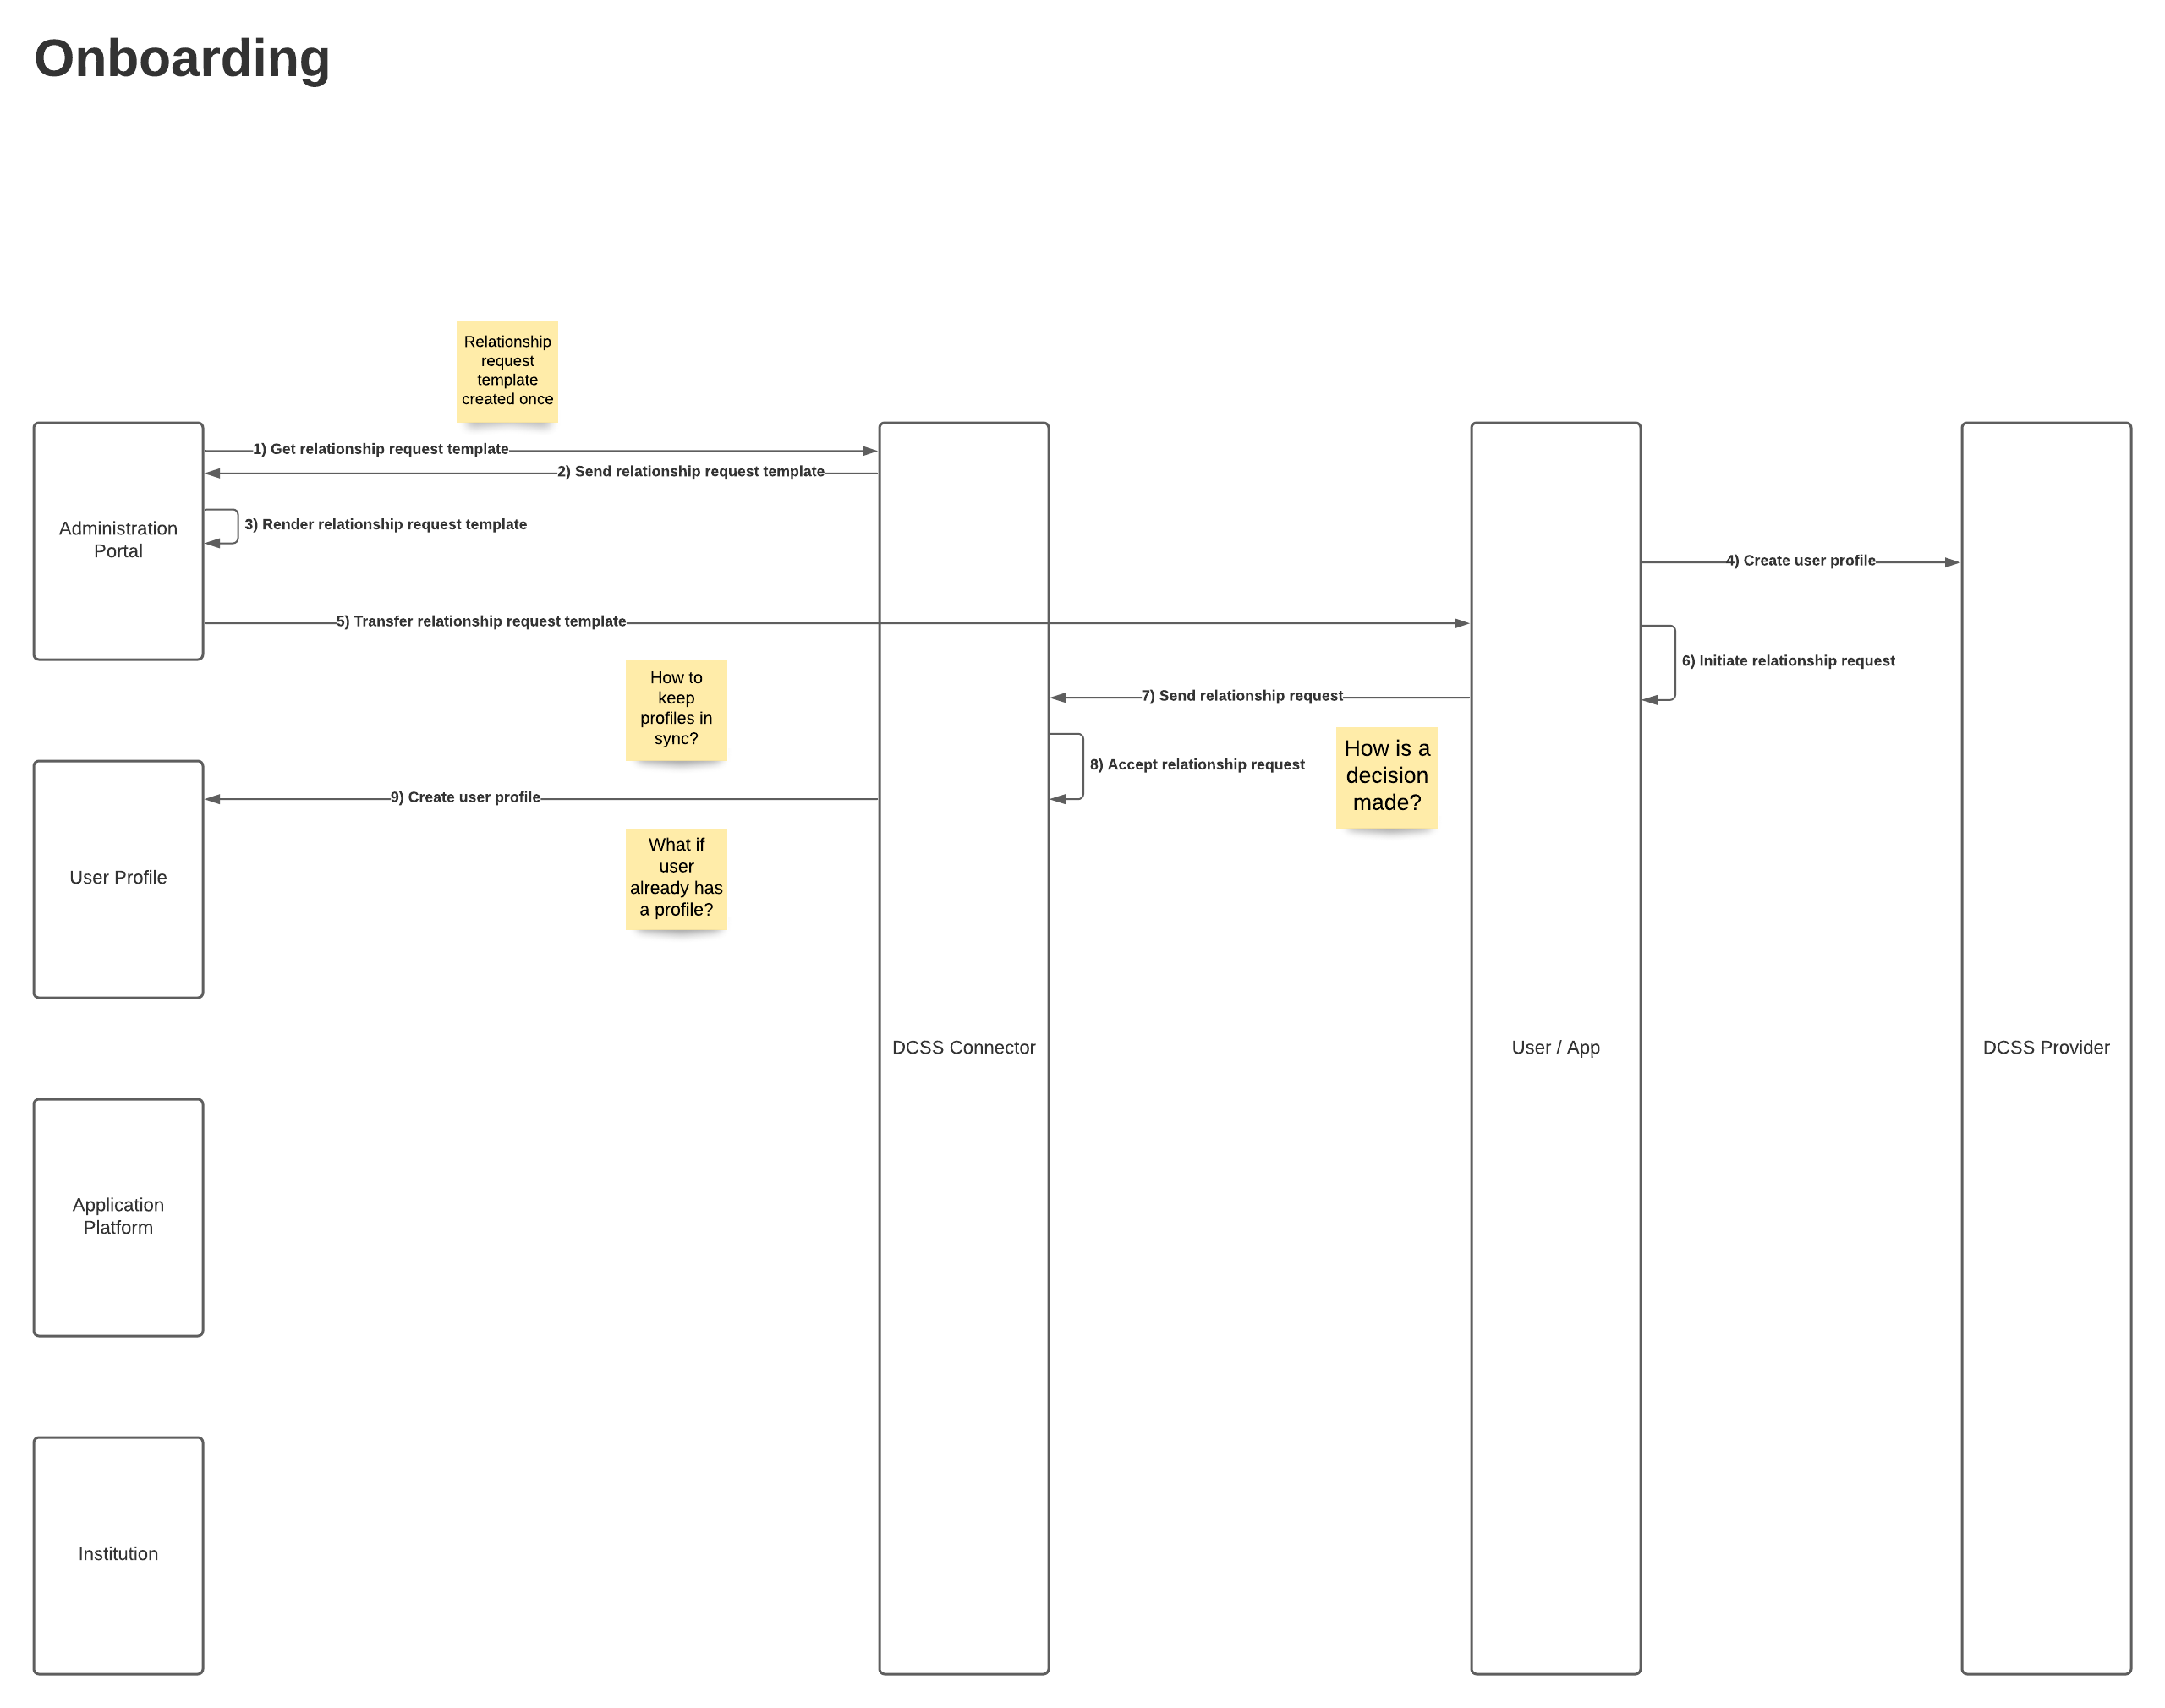
\includegraphics[width=15cm]{Basic Integration Onboarding.png}

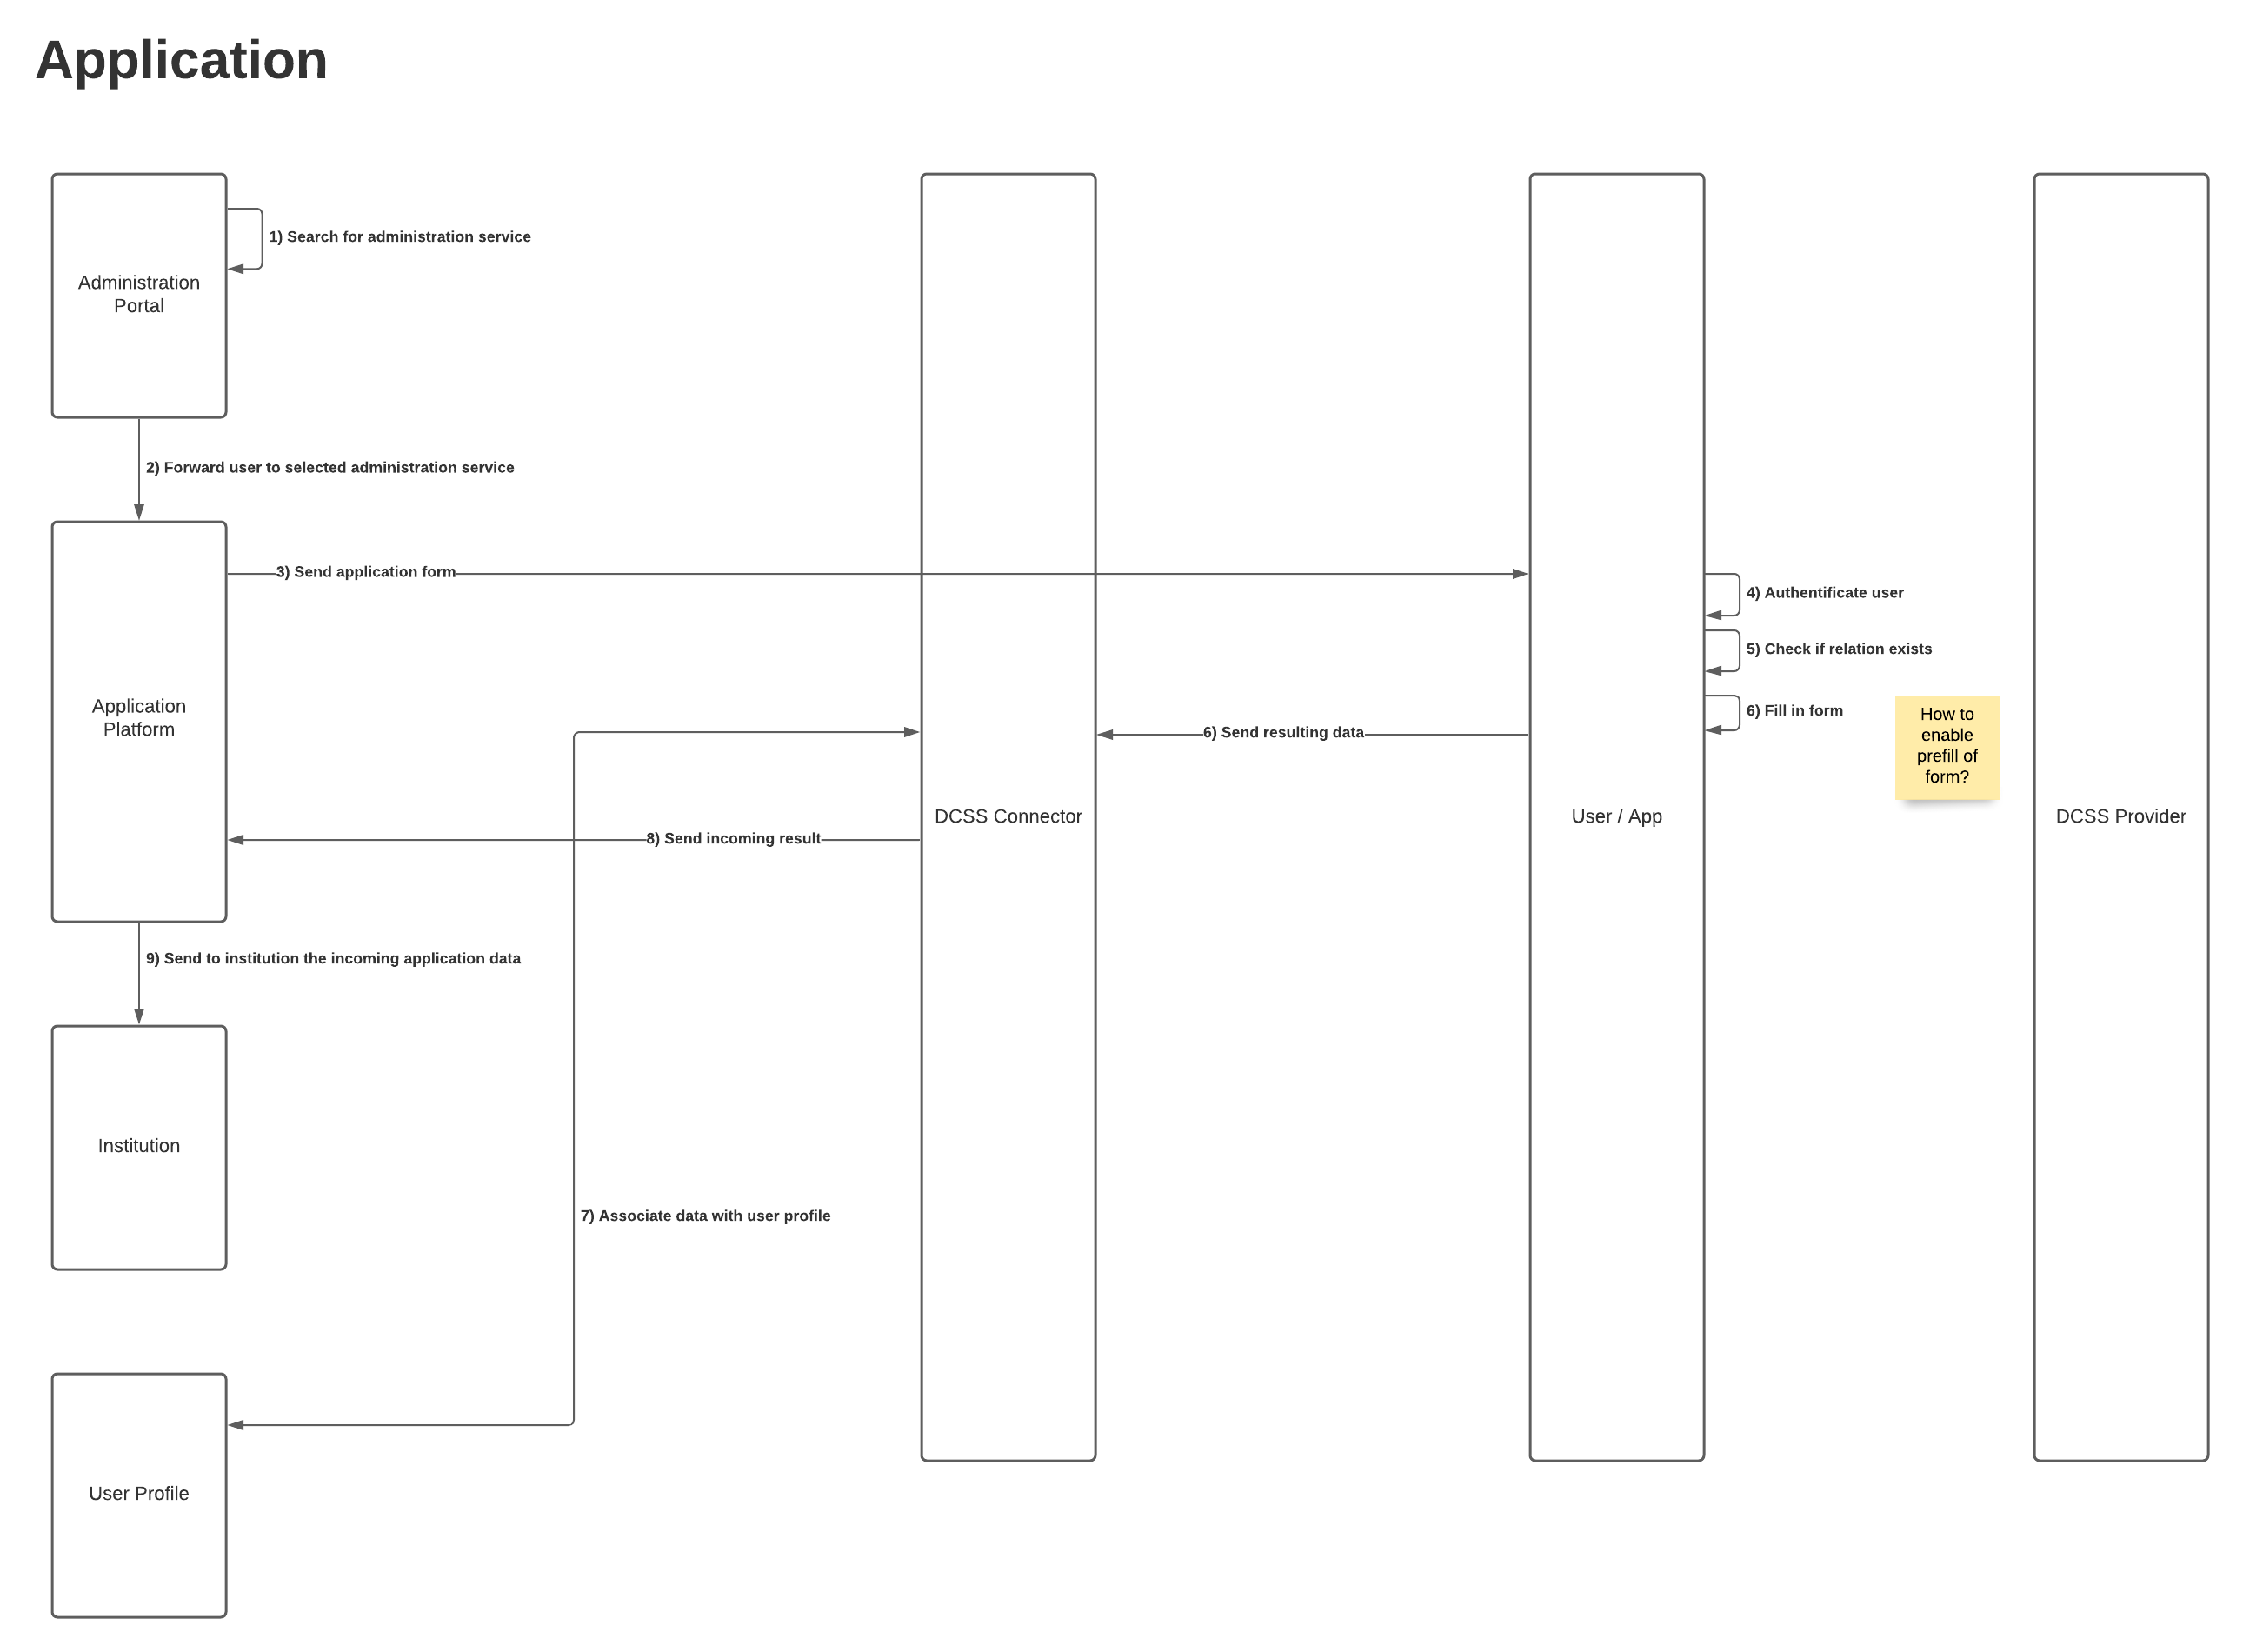
\includegraphics[width=15cm]{Basic Integration Application.png}

\subsubsection{Messaging Architecture}

\subsection{Version 2}

\subsubsection{Requirements}

\subsubsection{Flow Diagrams}

\subsubsection{Messaging Architecture}

\chapter{Solution Evaluation}

\section{Conclusion}

\chapter{Outlook}

\section{Advanced Integration Architecture}

\printbibliography


\end{document}
